\section{Theoretical Properties}
\label{sec:properties}
In this section, we see how the simplicity of the Elo-MMR formulas enables us to rigorously prove that the rating system is incentive-compatible, robust, and computationally efficient.

%\aram{erase this?} First, we discuss some properties that Elo-MMR has in common with the published systems of Codeforces and Topcoder, as well as the classical two-player systems Elo and Glicko. All of these systems propagate belief changes forward in time, never backward. This approach is simple, efficient, and has the benefit of never retroactively changing ratings from the past, nor the ratings of players who are not actively competing. In practice, Elo-MMR and Glicko also converge to the right results slightly faster than the others, by including an uncertainty parameter that starts high for new players.
\vspace{-.6em}
\subsection{Incentive-compatibility}
\label{sec:mono}

%\aram{erase this?} \emph{Aligned incentives} is one of our system's most important properties, so we devote this section to motivating, stating, and proving it. The main result, \Cref{thm:mono}, essentially guarantees that a player who seeks to improve their rating will never want to lose rounds, even if given the benefit of hindsight.

%To see that a "rational" rating system may fail monotonicity we begin with two examples.

%First, let's imagine a setting in which players typically maintain their "momentum"; that is, a player whose skill is improving rapidly, is expected to continue improving rapidly. A strategic player may then fake some momentum by intentionally performing at a weaker level, before returning to their actual level. The system may then believe that the player will continue to improve, granted inflated ratings until strong evidence arises to the contrary. This type of exploit was discovered in both the Topcoder rating system and the Pokemon Go rating system~\cite{forivsektheoretical, pokemongo}.%To show that this example is not just a hypothetical, \aram{cite Glicko-2, Topcoder, Pokemon Go}\cite{forivsektheoretical}.

%Next, we present a more subtle example. Consider a setting that presents players the choice between an easy challenge, which grants 1 point for partial success and 5 points for full success, or a hard challenge which grants 2 points for partial success and 10 points for full success.\footnote{This reward model is frequently used in coding competitions such as the International Olympiad of Informatics.} Experts with a high chance of a full success in the hard challenge should take it, whereas novices are likely to do better with the easy challenge. Let's suppose that, as a result, only experts attempt the hard challenges, and let's further suppose that a fraction of them fail to get a full success. Thus, there is a contingent of players with 2 points, all of whom are experts. If the rating system is powerful enough to know this, it may classify the 2-point players as stronger than the 5-point players, incentivizing a strategic novice to go for the lower point value!

%In summary, rating systems that are too powerful risk incentivizing players to perform cheap imitations of expert player behaviour, even when it undermines the game designer's objective for the player (e.g., to score more points). 

To demonstrate the need for incentive-compatibility, let's look at the consequences of violating this property in the Topcoder and Glicko-2 rating systems. These systems track a ``volatility'' for each player, which estimates the variance of their performances. A player whose recent performance history is more consistent would be assigned a lower volatility score, than one with wild swings in performance. The volatility acts as a multiplier on rating changes; thus, players with an extremely low or high performance will have their subsequent rating changes amplified.

While it may seem like a good idea to boost changes for players whose ratings are poor predictors of their performance, this feature has an exploit. By intentionally performing at a weaker level, a player can amplify future increases to an extent that more than compensates for the immediate hit to their rating. A player may even ``farm'' volatility by alternating between very strong and very weak performances. After acquiring a sufficiently high volatility score, the strategic player exerts their honest maximum performance over a series of contests. The amplification eventually results in a rating that exceeds what would have been obtained via honest play. This type of exploit was discovered in Glicko-2 as applied to the Pokemon Go video game~\cite{pokemongo}. Table 5.3 of ~\cite{forivsektheoretical} presents a milder violation in Topcoder competitions.

To get a realistic estimate of the severity of this exploit, we performed a simple experiment on the first five years of the Codeforces contest dataset (see \Cref{sec:datasets}). In \Cref{fig:topcoder-gaming}, we plot the rating evolution of the world's \#1 ranked competitive programmer, Gennady Korotkevich, better known as {\tt tourist}. In the \emph{control} setting, we plot his ratings according to the Topcoder and Elo-MMR($1$) systems. We contrast these against an \emph{adversarial} setting, in which we have {\tt tourist} employ the following strategy: for his first 45 contests, {\tt tourist} plays normally (exactly as in the unaltered data). For his next 45 contests, {\tt tourist} purposely falls to last place whenever his Topcoder rating is above 2975. Finally, {\tt tourist} returns to playing normally for an additional 15 contests.

This strategy mirrors the Glicko-2 exploit documented in~\cite{pokemongo}, and does not require unrealistic assumptions (e.g., we don't demand {\tt tourist} to exercise very precise control over his performances). Compared to a consistently honest {\tt tourist}, the volatility farming {\tt tourist} ended up \emph{523 rating points ahead} by the end of the experiment, with almost 1000 rating points gained in the last 15 contests alone. Transferring the same sequence of performances to the Elo-MMR($1$) system, we see that it not only is immune to such volatility-farming attacks, but it also penalizes the dishonest strategy with a rating loss that decays exponentially once honest play resumes.

\begin{figure}
\begin{minipage}{0.50\textwidth}
    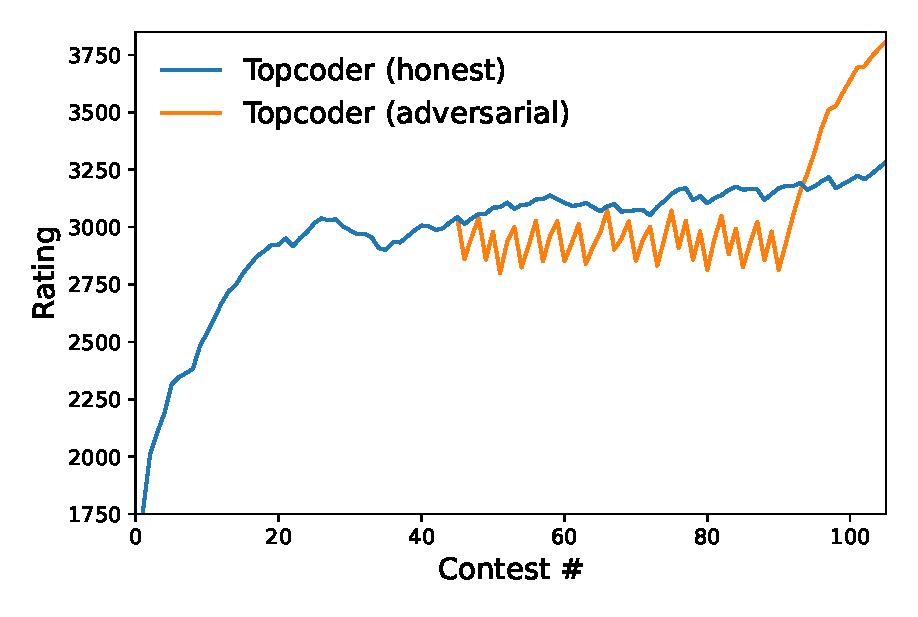
\includegraphics[width=0.95\textwidth]{images/topcoder.eps}
    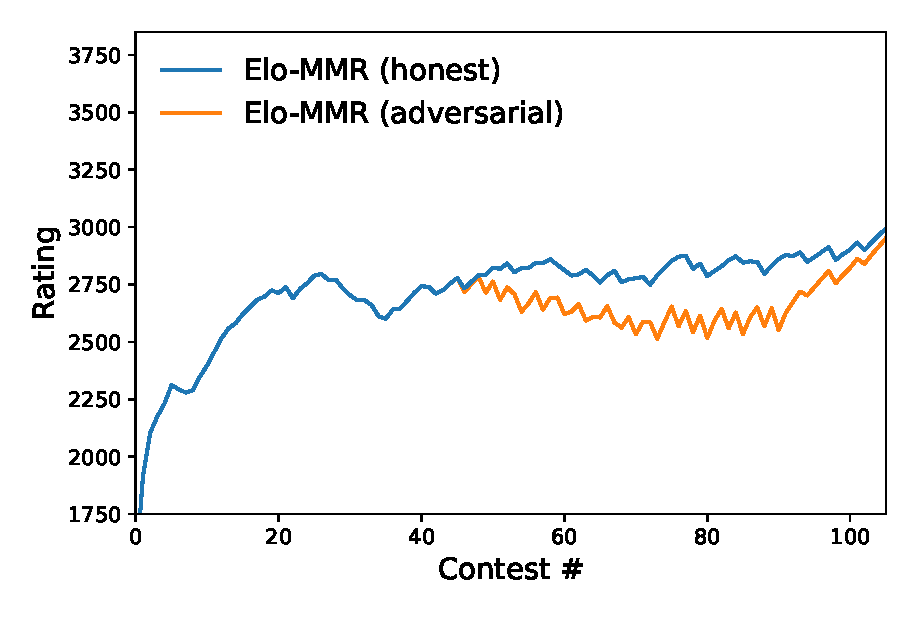
\includegraphics[width=0.95\textwidth]{images/elo-mmr.eps}
\end{minipage}
    \caption{Volatility farming attack on the Topcoder system.}
    \label{fig:topcoder-gaming}
\end{figure}

Recall that a key purpose of modeling volatility in Topcoder and Glicko-2 was to boost rating changes for inconsistent players. Remarkably, Elo-MMR achieves the same effect: we'll see in \Cref{sec:robust} that, for $\rho\in [0,\infty)$, Elo-MMR($\rho$) also boosts changes to inconsistent players. And yet, we'll now prove that no strategic incentive for purposely losing exists in \emph{any} version of Elo-MMR.

To this end, we need a few lemmas. Recall that, for the purposes of the algorithm, the performance $p_i$ is defined to be the unique zero of the function $Q_i(p) := \sum_{j \succ i} l_j(p) + \sum_{j \sim i} d_j(p) + \sum_{j \prec i} v_j(p)$, whose terms $l_i,d_i,v_i$ are contributed by opponents against whom $i$ lost, drew, or won, respectively. Wins (losses) are always positive (negative) contributions to a player's performance score:
\begin{lemma}
\label{lem:mono-term}
Adding a win term to $Q_i(\cdot)$, or replacing a tie term by a win term, always increases its zero. Conversely, adding a loss term, or replacing a tie term by a loss term, always decreases it.
\end{lemma}

\begin{proof}
By \Cref{lem:decrease}, $Q_i(p)$ is decreasing in $p$. Thus, adding a positive term will increase its zero whereas adding a negative term will decrease it. The desired conclusion follows by noting that, for all $j$ and $p$, $v_j(p)$ and $v_j(p)-d_j(p)$ are positive, whereas $l_j(p)$ and $l_j(p)-d_j(p)$ are negative.
\end{proof}

While not needed for our main result, a similar argument shows that performance scores are monotonic across the round standings:

\begin{theorem}
If $i \succ j$ (that is, player $i$ beats $j$) in a given round, then player $i$ and $j$'s performance estimates satisfy $p_i > p_j$.
\end{theorem}

\begin{proof}
If $i \succ j$ with $i,j$ adjacent in the rankings, then
\[Q_i(p) - Q_j(p) = \sum_{k\sim i}(d_k(p) - l_k(p)) + \sum_{k\sim j}(v_k(p) - d_k(p)) > 0.\]
for all $p$. Since $Q_i$ and $Q_j$ are decreasing functions, it follows that $p_i > p_j$. By induction, this result extends to the case where $i,j$ are not adjacent in the rankings.
\end{proof}

What matters for incentives is that performance scores be \emph{counterfactually} monotonic; meaning, if we were to alter the round standings, a strategic player will always prefer to place higher:
\begin{lemma}
\label{lem:mono-perf}
In any given round, holding fixed the relative ranking of all players other than $i$ (and holding fixed all preceding rounds), the performance $p_i$ is a monotonic function of player i's prior rating and of player $i$'s rank in this round.
\end{lemma}

\begin{proof}
Monotonicity in the prior rating follows directly from monotonicity of the self-tie term $d_i$ in $Q_i$. Since an upward shift in the rankings can only convert losses to ties to wins, monotonicity in contest rank follows from \Cref{lem:mono-term}. 
\end{proof}

Having established the relationship between round rankings and performance scores, the next step is to prove that, even with hindsight, players will always prefer their performance scores to be as high as possible:

\begin{lemma}
\label{lem:mono-rate}
Holding fixed the set of contest rounds in which a player has participated, their current rating is monotonic in each of their past performance scores.
\end{lemma}

\begin{proof}
The player's rating is given by the zero of $L'$ in \Cref{eq:multiplicities}. The pseudodiffusions of \Cref{sec:skill-drift} modify each of the $\beta_k$ in a manner that does not depend on any of the $p_k$, so they are fixed for our purposes. Hence, $L'$ is monotonically increasing in $s$ and decreasing in each of the $p_k$. Therefore, its zero is monotonically increasing in each of the $p_k$.

This is almost what we wanted to prove, except that $p_0$ is not a performance. Nonetheless, it is a function of the performances: specifically, a weighted average of historical ratings which, using this same lemma as an inductive hypothesis, are themselves monotonic in past performances. By induction, the proof is complete.
\end{proof}

Finally, we conclude that a rating-maximizing player is always motivated to improve their round rankings, or raw scores:

\begin{theorem}[Incentive-compatibility]
\label{thm:mono}
Holding fixed the set of contest rounds in which each player has participated, and the historical ratings and relative rankings of all players other than $i$, player $i$'s current rating is monotonic in each of their past rankings.
\end{theorem}

\begin{proof}
Choose any contest round in player $i$'s history, and consider improving player $i$'s rank in that round while holding everything else fixed. It suffices to show that player $i$'s current rating would necessarily increase as a result.

In the altered round, by \Cref{lem:mono-perf}, $p_i$ is increased; and by \Cref{lem:mono-rate}, player $i$'s post-round rating is increased. By \Cref{lem:mono-perf} again, this increases player $i$'s performance score in the following round. Proceeding inductively, we find that performance scores and ratings from this point onward are all increased.
\end{proof}

In the special cases of Elo-MM$\chi$ or Elo-MMR($\infty$), the rating system is ``memoryless'': the only data retained for each player are the current rating $\mu_{i,t}$ and uncertainty $\sigma_{i,t}$; detailed performance history is not saved. In this setting, we present a natural monotonicity theorem. A similar theorem was previously stated for the Codeforces system, albeit in an informal context without proof~\cite{Codeforces}.

\begin{theorem}[Memoryless Monotonicity]
In either the Elo-MM$\chi$ or Elo-MMR($\infty$) system, suppose $i$ and $j$ are two participants of round $t$. Suppose that the ratings and corresponding uncertainties satisfy $\mu_{i,t-1} \ge \mu_{j,t-1},\; \sigma_{i,t-1} = \sigma_{j,t-1}$. Then, $\sigma_{i,t} = \sigma_{j,t}$. Furthermore:

If $i \succ j$ in round $t$, then $\mu_{i,t} > \mu_{j,t}$.

If $j \succ i$ in round $t$, then $\mu_{j,t} - \mu_{j,t-1} > \mu_{i,t} - \mu_{i,t-1}$.
\end{theorem}

\begin{proof}
The new contest round will add a rating perturbation with variance $\gamma_t^2$, followed by a new performance with variance $\beta_t^2$. As a result,
\[\sigma_{i,t}
= \left( \frac{1}{\sigma_{i,t-1}^2 + \gamma_t^2} + \frac{1}{\beta_t^2} \right)^{-\frac 12}
= \left( \frac{1}{\sigma_{j,t-1}^2 + \gamma_t^2} + \frac{1}{\beta_t^2} \right)^{-\frac 12}
= \sigma_{j,t}.\]

The remaining conclusions are consequences of three properties: memorylessness, incentive-compatibility (\Cref{thm:mono}), and translation-invariance (ratings, skills, and performances are quantified on a common interval scale relative to one another).

Since the Elo-MM$\chi$ or Elo-MMR($\infty$) systems are memoryless, we may replace the initial prior and performance histories of players with any alternate histories of our choosing, as long as our choice is compatible with their current rating and uncertainty. For example, both $i$ and $j$ can be considered to have participated in the same set of rounds, with $i$ always performing at $\mu_{i,t-1}$. and $j$ always performing at $\mu_{j,t-1}$. Round $t$ is unchanged.

Suppose $i \succ j$. Since $i$'s historical performances are all equal or stronger than $j$'s, \Cref{thm:mono} implies $\mu_{i,t} > \mu_{j,t}$.

Suppose $j \succ i$. By translation-invariance, if we shift each of $j$'s performances, up to round $t$ and including the initial prior, upward by $\mu_{i,t-1} - \mu_{j,t-1}$, the rating changes between rounds will be unaffected. Players $i$ and $j$ now have identical histories, except that we still have $j\succ i$ at round $t$. Therefore, $\mu_{j,t-1} = \mu_{i,t-1}$ and, by \Cref{thm:mono}, $\mu_{j,t} > \mu_{i,t}$. Subtracting the equation from the inequality proves the second conclusion.
\end{proof}

\subsection{Robust response}
\label{sec:robust}

Another desirable property in many settings is robustness: a player's rating should not change too much in response to any one contest, no matter how extreme their performance. The Codeforces and TrueSkill systems lack this property, allowing for unbounded rating changes. Topcoder achieves robustness by clamping any changes that exceed a cap, which is initially high for new players but decreases with experience.

When $\rho>0$, Elo-MMR($\rho$) achieves robustness in a natural, smoother manner. To understand how, we look at the interplay between Gaussian and logistic factors in the posterior. Recall the notation in \Cref{eq:multiplicities}, describing the loss function and weights.

\begin{theorem}
\label{thm:robust}
In the Elo-MMR($\rho$) rating system, let
\[\Delta_+ := \lim_{p_t\rightarrow+\infty} \mu_{t}-\mu_{t-1},
\quad\Delta_- := \lim_{p_t\rightarrow-\infty}\mu_{t-1}-\mu_{t}.
\]
Then, for $\Delta_\pm \in \{\Delta_+, \Delta_-\}$,
\[\frac{\pi}{\beta_t\sqrt 3}
\left(w_0 + \frac{\pi^2}{6}\sum_{k\in\cH_{t-1}}w_k \right)^{-1}
\le \Delta_\pm
\le \frac{\pi}{\beta_t\sqrt 3}\frac{1}{w_0}.\]
%Then $\Delta_{min} \le \Delta < \Delta_{max}$, where
%\begin{align*}
%\Delta_{min} + \frac{2\pi\beta_t\beta_0^2}{\sqrt 3}(\sum_{k\in\mathcal R}\frac{1}{\beta_k})\tanh\frac{\Delta_{min}\pi}{4\sqrt 3 \beta_t} &= \frac{\pi\beta_0^2}{\beta_t\sqrt 3}
%\\\Delta_{max} &= \frac{\pi\beta_0^2}{\beta_t\sqrt 3}
%\end{align*}
\end{theorem}

\begin{proof}
Using the fact that $0 < \frac{d}{dx}\tanh(x) \le 1$, differentiating $L'$ in \Cref{eq:multiplicities} yields
\[\forall s\in\mathbb R,\; w_0 \le L''(s)
\le w_0 + \frac{\pi^2}{6}\sum_{k\in\cH_{t-1}}w_k.\]

Now, the performance at round $t$ adds a new term with multiplicity one to $L'(s)$: its value is
$\frac{\pi}{\beta_k\sqrt{3}} \tanh \frac{(s-p_k)\pi}{\beta_k\sqrt{12}}$.

As a result, for every $s\in\mathbb R$, in the limit as $p_t\rightarrow\pm\infty$, $L'(s)$ increases by $\mp\frac{\pi}{\beta_t\sqrt 3}$. Since $\mu_{t-1}$ was a zero of $L'$ without this new term, we now have
$L'(\mu_{t-1}) \rightarrow \mp\frac{\pi}{\beta_t\sqrt 3}.$ Dividing by the former inequalities yields the desired result.
\end{proof}

The proof reveals that the magnitude of $\Delta_{\pm}$ depends inversely on that of $L''$ in the vicinity of the current rating, which in turn is related to the derivative of the $\tanh$ terms. If a player's performances vary wildly, the tanh terms will be widely dispersed, so any potential rating value will necessarily be in the tail ends of most of the terms. Tails contribute very small derivatives, enabling a larger rating change. Conversely, the $\tanh$ terms of a player with a very consistent performance history will contribute large derivatives, so the bound on their rating change will be small.

Thus, Elo-MMR naturally caps the rating changes of all players, and the cap is smaller for consistent performers. The cap will increase after an extreme performance, providing a similar ``momentum'' to the Topcoder and Glicko-2 systems, but without sacrificing incentive-compatibility (\Cref{thm:mono}).

We can compare the lower and upper bound in \Cref{thm:robust}: their ratio is on the same order as the fraction of the total weight that is held by the normal term. Recall that $\rho$ is the weight transfer rate: larger $\rho$ results in more weight being transferred into $w_0$; in this case, the lower and upper bound tend to stay close together. Conversely, the momentum effect is more pronounced when $\rho$ is small. In the extreme case $\rho=0$, $w_0$ vanishes for experienced players, so a sufficiently volatile player would be subject to correspondingly large rating updates. In the extended version of this paper, we quantify an asymptotic steady state for the weights, and argue that $1/\rho$ can be thought of as a momentum parameter.

\subsection{Runtime analysis and optimizations}
\label{sec:runtime}
Let's look at the computation time needed to process a round with participant set $\mathcal P$, where we again omit the round subscript. Each player $i$ has a participation history $\cH_i$.

Estimating $P_i$ entails finding the zero of a monotonic function with $O(|\mathcal P|)$ terms, and then obtaining the rating $\mu_i$ entails finding the zero of another monotonic function with $O(|\cH_i|)$ terms. Using either of the Illinois or Newton methods, solving these equations to precision $\epsilon$ takes $O(\log\log\frac 1\epsilon)$ iterations. As a result, the total runtime needed to process one round of competition is
\[O\left(\sum_{i\in\mathcal P}(|\mathcal P| + |\cH_i|) \log\log\frac 1\epsilon\right).\]
This complexity is more than adequate for Codeforces-style competitions with thousands of contestants and history lengths up to a few hundred. Indeed, we were able to process the entire history of Codeforces on a small laptop in less than half an hour. Nonetheless, it may be cost-prohibitive in truly massive settings, where $|\mathcal P|$ or $|\cH_i|$ number in the millions. Fortunately, it turns out that both functions may be compressed down to a bounded number of terms, with negligible loss of precision.

\paragraph{Adaptive subsampling}
In \Cref{sec:bayes_model}, we used Doob's consistency theorem to argue that our estimate for $P_i$ is consistent. Specifically, we saw that $O(1/\epsilon^2)$ opponents are needed to get the typical error below $\epsilon$. Thus, we can subsample the set of opponents to include in the estimation, omitting the rest. Random sampling is one approach. A more efficient approach chooses a fixed number of opponents whose ratings are closest to that of player $i$, as these are more likely to provide informative match-ups. On the other hand, if the setting requires incentive-compatibility to hold exactly, then one must avoid choosing different opponents for each player.

\paragraph{History compression}
Similarly, it's possible to bound the number of stored factors in the posterior. Our skill-evolution algorithm decays the weights of old performances at an exponential rate. Thus, the contributions of all but the most recent $O(\log\frac 1\epsilon)$ terms are negligible. Rather than erase the older logistic terms outright, we recommend replacing them with moment-matched Gaussian terms, similar to the transfers in \Cref{sec:skill-drift} with $\kappa_t=0$. Since Gaussians compose easily, a single term can then summarize an arbitrarily long prefix of the history.

Substituting $1/\epsilon^2$ and $\log\frac 1\epsilon$ for $|\cP|$ and $|\cH_i|$, respectively, the runtime of Elo-MMR with both optimizations becomes
\[O\left(\frac {|\mathcal P|}{\epsilon^2} \log\log\frac 1\epsilon\right).\]

If the contests are \emph{extremely large}, so that $\Omega(1/\epsilon^2)$ opponents have a rating and uncertainty in the same $\epsilon$-width bucket as player $i$, then it's possible to do even better: up to the allowed precision $\epsilon$, the corresponding terms can be treated as duplicates. Hence, their sum can be determined by counting how many of these opponents win, lose, or tie against player $i$. Given the pre-sorted list of ranks of players in the bucket, two binary searches would yield the answer. In practice, a single bucket might not contain enough participants, so we sample enough buckets to yield the desired precision.

\paragraph{Simple parallelism}
Since each player's rating computation is independent, the algorithm is embarrassingly parallel. Threads can read the same global data structures, so each additional thread contributes only $O(1)$ memory overhead.

% \subsection{erase all this, or present in a different way?}

% Imagine a player who performs very consistently over a long period of time, repeatedly achieving $p_i = 1000$ until convergence. Now, perhaps as a result of attending an intensive training camp in Petrozavodsk, their skill changes dramatically. From this point on, they consistently achieve $p_i = 3000$.

% How does each rating system respond to the first such surprise occurrence? Elo-MMR treats the new result as a fluke, an outlier that ought to be ignored. The player gains 48 points; as a result of the parameters we set, this is the maximum possible for an experienced player as $p_i \rightarrow \infty$. In practice, ratings may change by more than 48, as the maximum depends on existing fluctuations in their history; here we're looking at the extreme example of a player with a history of always performing at exactly $p_i = 1000$.

% \begin{figure}
%     \centering
%     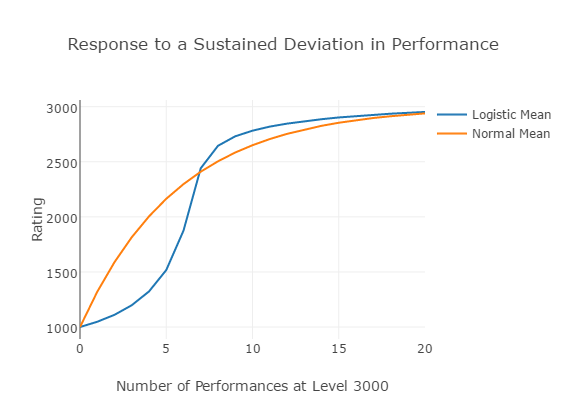
\includegraphics[width=\columnwidth]{images/ResponsePlot.png}
%     \caption{An accelerated convergence effect in the presence of sustained improved performances.}
%     \label{fig:accelerated}
% \end{figure}

% Had we tried to perform outlier reduction in a memoryless fashion, we would continue to increase the rating by 48 per match, oblivious to the possibility that the player truly did experience a sudden improvement. In Elo-MMR, the outlier status of a performance is treated as tentative. If later matches support the hypothesis of having improved, the rating will increase by an additional 63 points, followed by over 100 points in each of the third and following matches, as plotted by the blue curve above.

% After six consecutive matches with $p_i = 3000$, the rating is 1875 and very unstable (even though $\sigma_i$ is unchanged!). The system is no longer sure which to trust: the extensive history at level 1000, or the smaller number of recent matches at level 3000. Depending on what comes next, the player's rating can very quickly fall toward 1000 or rise toward 3000. However, note that in either case, the change will not overshoot, say to 5000, unless enough new evidence is accumulated at that level. As the $p_i=3000$ streak continues, the seventh match on the blue curve jumps by a whopping 566 points. As the player's rating converges to 3000, the old $p_i = 1000$ data acquires outlier status, thus speeding convergence.

% In contrast, while a system such as Codeforces does not compute $p_i$ values in quite in the same way, we can obtain a good approximation by removing outlier reduction from Elo-MMR, effectively treating the performances to be averaged as normal instead of logistic measurements. This makes the system effectively memoryless, since it turns out that each match simply moves the rating about 16\% closer to the new $p_i$ value, independent of the history. With this change, we obtain the orange curve, which jumps a whopping 320 points at the very first performance. Indeed, there is no limit: if you could find players whose ratings are extremely high, and beat them even once, your rating would take arbitrarily large leaps.

% Note that this is not quite true of Topcoder, which incorporates a hack that caps the maximum rating change: if Topcoder's update formula demands too large a change, the cap kicks in. In contrast, Elo-MMR's cap is a natural and smooth consequence of its update formula and is sensitive to whether a change is charting new territory, or merely confirming a plausible hypothesis. Topcoder does attempt to make the magnitude of its updates sensitive to the amount of fluctuation in a player's history, using a volatility measure, but this measure does not account for the direction of the changes, resulting in the non-monotonicity flaw mentioned above.

% Notwithstanding arguments that a high rating ought to properly be earned over multiple matches rather than a single fluke, the other danger is that these observations also hold in reverse: one bad day on Codeforces can seriously damage one's rating and negate several rounds of steady progress. By using heavy-tailed logistic distributions everywhere, Elo-MMR understands that unusually high or low performances do occasionally occur, and one round in isolation is never a reliable signal.

% Interestingly, despite the slow start, the blue curve ultimately converges faster than the orange one. Since Elo-MMR uses its memory to dynamically adapt its view of potential outliers, it overtakes the orange curve as soon as new evidence outweighs the old hypothesis!

% \subsection{Inflation and division boundary artifacts: erase or rewrite?}

% The code and ratings of real Codeforces members as computed by Elo-MMR are available at https://github.com/EbTech/EloR. Original Codeforces ratings are at http://codeforces.com/ratings. One striking difference is massive inflation in the Codeforces system. Gennady Korotkevich, best known by his competitive programming handle ``tourist'', has been the reigning world champion for years. Toward the end of 2011, his rating reached a new ceiling of about 2700 according to both systems. However, as of this writing, his rating on Elo-MMR has increased by about 300 additional points, while on Codeforces it increased by almost 900. To get a sense of the magnitude of this change, 900 points is the difference between an average member and a Grandmaster! Indeed, most of the variance in the Codeforces system is concentrated at the top, with much smaller rating differences between beginner and intermediate members. This is caused by certain ad hoc elements of the system that are not founded on any rigorous model.